\subsection{Example}

Let us present a solution of motivating example: grammar $G_1$ is a query and we want to find all paths in graph $M$ (presented in picture~\ref{input}) matching this query.
Result SPPF for this input is presented in figure~\ref{SPPF}. Note that presented version does not contains redundant nodes.
Each terminal node corresponds to the edge in the input graph: for each node with label $(v_0, T, v_1)$ there is $e\in E: e=(v_0,T,v_1)$.
We duplicate terminal nodes only for figure simplification.

\begin{figure}[h]
    \begin{center}
        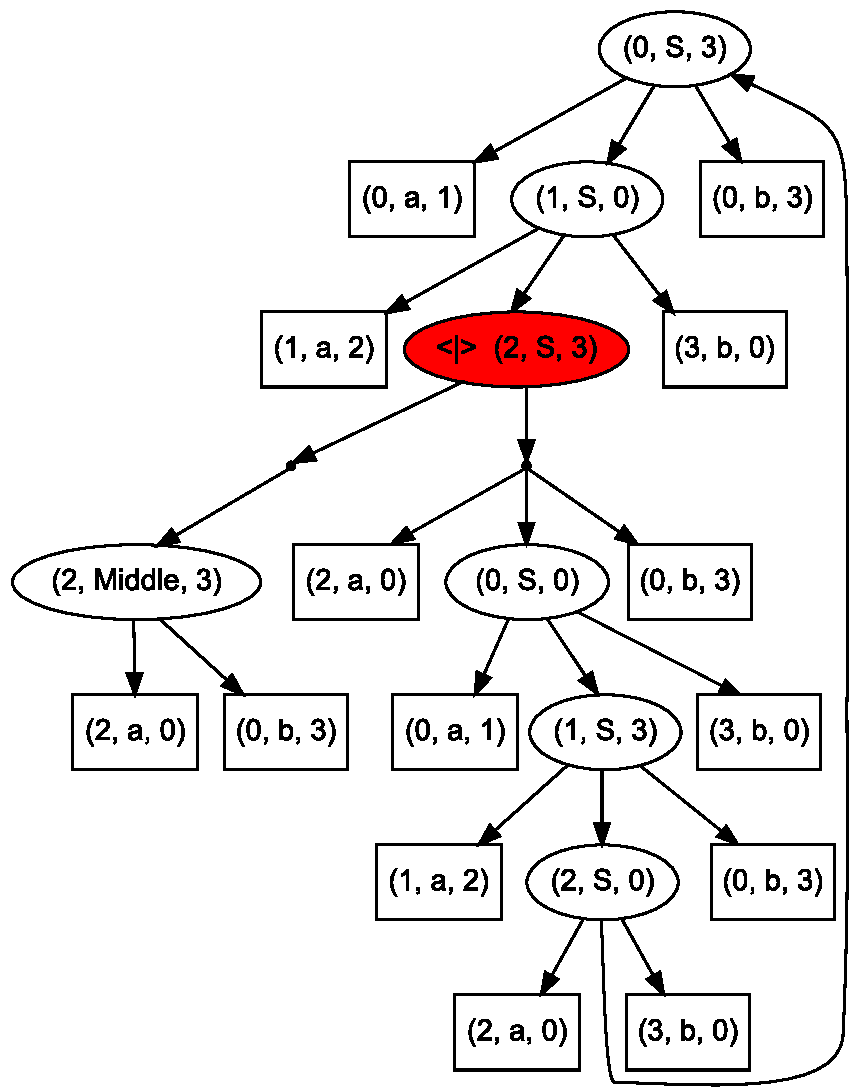
\includegraphics[width=8cm]{dot/AnBn.pdf}
        \caption{Result SPPF for input graph $M$(fig.~\ref{input}) and query $G_1$(fig.~\ref{grammarG})}
        \label{SPPF}        
    \end{center}
\end{figure}

    
As an example of derivation structure usage we can find 'middle' of any path in example above simply by finding correspondent nonterminal \textit{Middle} in SPPF.
So we can find out that there is only one common ancestor for all results, and it is a vertex with $id = 0$. 

Extensions stored in nodes allow us to check whether path from $u$ to $v$ exists, and to extract it. 
To extract specified path we need only to traverse SPPF, and it can be done in linear time (in terms of SPPF size). 

Lets find paths satisfying specified in $G_1$ constraints from vertex $0$.
To do this, we should find vertices with label $(0, S, \_)$ in SPPF.
We can see that there are two vertices with label matched this pattern: $(0, S, 0)$ and $(0, S, 3)$.
At the next step let us to extract corresponded paths from SPPF.
In our example there is a cycle in SPPF so there are \textbf{at least} two different paths: $$p_0=\{(0,a,1);(1,a,2);(2,a,0);(0,b,3);(3,b,0);(0,b,3)\}$$ and 
\begin{align*}
p_1=\{&(0,a,1);(1,a,2);(2,a,0);(0,a,1);(1,a,2);(2,a,0);\\ &(0,b,3);(3,b,0);(0,b,3);(3,b,0);(0,b,3);(3,b,0)\}.
\end{align*}


Thus SPPF which was constructed by described algorithm can be useful for query result investigation. 
But in some cases explicit representation of matched subgraph is preferable, and required subgraph that may be extracted from SPPF trivially by its traversal.
